\section{Rezultati}

\subsection{Simulacije}
Skupno smo izvedli 6000 simulacij. Tri tisoč simulacij smo izvedli na način, da smo individualno spremenljivko izračunali s pomočjo simuliranih vrednosti standardnega odklona (normalna porazdelitev) in na podlagi vzorčenih točk izračunanim centroidom kot povprečje ($\mu$). S pomočjo programa MARK smo uspešno ocenili v 2916 simulacijah.
Enako število simulacij smo izvedli za primer, kjer smo krivuljo za izračun individualne spremenljivke ocenili iz podatkov (empirična porazdelitev). Pri oceni parametrov smo bili uspešni 2681-krat (Tabela \ref{tab:tabela1}).

Da nekaterih modelov nismo uspešno ocenili je po pričakovanjih. Zaradi določene strukture podatkov je možno, da optimizacijski kriterij znotraj parametrskega prostora ne najde optimuma, ali pa so ocenjeni parametri na intervalu $- \infty < x < \infty$. Tiste simulacije, ki niso dale smiselnega rezultata, smo iz analize izključili.

Na polno obremenjenem računalniku je bila simulacija izračuna individualne spremenljivke končana v približno 48 urah. Nadaljnje analize ulova in ponovnega ulova ter priprava podatkov za analizo pa so zahtevale še dodatnih šest ur.

Zaznati je mogoče vzorec v številu uspešnih simulacij glede na uporabljeno funkcijo. Število uspešnih simulacij glede na število generiranih osebkov in število odlovnih intervalov se med tema dvema skupinama razlikuje. Večina neuspelih simulacij pri uporabi empirične funkcije je za najmanjše število odlovnih intervalov ($K=5$).

\begin{table}[!htb]
  \caption{Prikaz števila simulacij, kjer smo uspešno ocenili parametre, glede na funkcijo, ki je bila uporabljena za izračun individualne spremenljivke. V vrsticah je število generiranih osebkov ($N$), v stolpcih pa število odlovnih intervalov ($K$). Uspešno izračunanih simulacij z empirično funkcijo je nekoliko manj. Za lažjo predstavo v spodnji matriki prikazujemo razliko med zgornjima tabelama tako, da smo empirični (levo) odšteli normalno (desno) tabelo. Pretežni delež neuspelih simulacij je predvsem na račun simulacij, ki imajo 5 odlovnih intervalov in/ali manjše število simuliranih osebkov (nižja gostota).}
  \label{tab:tabela1}
\begin{tabular}{cc}
    \begin{minipage}{.33\linewidth}
      \caption*{Empirična funkcija}
      \resizebox{\columnwidth}{!}{%
        \begin{tabular}{rccc}
          \toprule
           & \textbf{$K=5$} & \textbf{$k=10$} & \textbf{$K=15$} \\
          \midrule
          $N=500$ & 142 & 187 & 190 \\
          $N=800$ & 141 & 192 & 178 \\
          $N=1000$ & 135 & 182 & 185 \\
          $N=1300$ & 168 & 212 & 194 \\
          $N=1500$ & 171 & 186 & 218 \\
          \bottomrule
        \end{tabular}
        }
    \end{minipage}%

    \begin{minipage}{.33\linewidth}
      \caption*{Normalna funkcija}
      \resizebox{\columnwidth}{!}{%
        \begin{tabular}{rccc}
          \toprule
           & \textbf{$K=5$} & \textbf{$k=10$} & \textbf{$K=15$} \\
          \midrule
          $N=500$ & 188 & 209 & 197 \\
          $N=800$ & 179 & 205 & 183 \\
          $N=1000$ & 175 & 190 & 185 \\
          $N=1300$ & 191 & 212 & 195 \\
          $N=1500$ & 199 & 190 & 218 \\
          \bottomrule
        \end{tabular}
        }
    \end{minipage}%

    \begin{minipage}{.33\linewidth}
      \caption*{Razlike med matrikama}
      \resizebox{\columnwidth}{!}{%
        \begin{tabular}{rccc}
          \toprule
           & \textbf{$K=5$} & \textbf{$k=10$} & \textbf{$K=15$} \\
          \midrule
          $N=500$ & -46 & -22 & -7 \\
          $N=800$ & -38 & -13 & -5 \\
          $N=1000$ & -40 & -8 & 0 \\
          $N=1300$ & -23 & 0 & -1 \\
          $N=1500$ & -28 & -4 & 0 \\
          \bottomrule
        \end{tabular}
        }
    \end{minipage}
\end{tabular}
\end{table}

\subsection{Parameter p modelov $M_0$ in $M_{sp}$ po Hugginsu}
Za modela $M_0$ in Msp modelu smo predpostavili, da sta parametra $p$ in $c$ enaka. Ulovljivost v prvem in vseh ostalih odlovnih presledkih predpostavljamo enako. Zato v analizi obravnavamo le parameter ulovljivosti $p$. Za lažjo primerjavo smo izračunali razmerje med ocenjeno in simulirano vrednostjo $p$ (slika \ref{sli:slika3}). Model TIRM oceni $p$ za dve skupini, kar neposredno ni primerljivo s parametrom $p$ po Hugginsovem modelu, zato le-tega nismo podrobneje preučili.

V povprečju je ulovljivost za vse simulacije in modele podcenjena in je približno med 0.35 in 0.4 deleža simulirane vrednosti. Ulovljivost ocenjena po modelu Msp je nekoliko bolj podcenjena, ne glede na to s pomočjo katere porazdelitve izračunamo individualno spremenljivko. V povprečju je ulovljivost za primer empirične porazdelitve za oba modela nekoliko nižja (za približno 0.01). Vidimo tudi, da se razlika med modeloma rahlo zmanjša s povečanjem simulirane ulovljivosti (slika \ref{sli:slika3}).

\subsubsection{Primerjava simulirane in ocenjene ulovljivosti glede na porazdelitev}
\subsubsubsection{Empirična porazdelitev}
Povprečje deleža simulirane vrednosti preprostega $M_0$ modela je 0.397, modela z individualno spremenljivko $M_{sp}$ pa za 0.035 nižja.

\begin{verbatim}
Call:
glm(formula = p.val ~ p.var, data = xep)

Deviance Residuals:
 	Min    	1Q	Median    	3Q   	Max
-0.36868  -0.16667  -0.07254   0.09971   1.44373

Coefficients:
              	Estimate Std. Error t value Pr(>|t|)
(Intercept)   	0.397081   0.001467  270.69   <2e-16 ***
p.varp.target.sp -0.035010   0.002075  -16.88   <2e-16 ***
---
Signif. codes:  0 ‘***’ 0.001 ‘**’ 0.01 ‘*’ 0.05 ‘.’ 0.1 ‘ ’ 1

(Dispersion parameter for gaussian family taken to be 0.05769313)

	Null deviance: 3109.8  on 53619  degrees of freedom
Residual deviance: 3093.4  on 53618  degrees of freedom
AIC: -786.36
\end{verbatim}

\subsubsubsection{Normalna porazdelitev}
Povprečje deleža simulirane vrednosti preprostega $M_0$ modela je 0.387, modela z individualno spremenljivko $M_{sp}$ pa 0.349 (0.038 nižja).

\begin{verbatim}
Call:
glm(formula = p.val ~ p.var, data = xep)

Deviance Residuals:
 	Min    	1Q	Median    	3Q   	Max
-0.35876  -0.16239  -0.07163   0.09433   1.45364

Coefficients:
              	Estimate Std. Error t value Pr(>|t|)
(Intercept)   	0.387167   0.001381  280.29   <2e-16 ***
p.varp.target.sp -0.037886   0.001953  -19.39   <2e-16 ***
---
Signif. codes:  0 ‘***’ 0.001 ‘**’ 0.01 ‘*’ 0.05 ‘.’ 0.1 ‘ ’ 1

(Dispersion parameter for gaussian family taken to be 0.05563641)

	Null deviance: 3265.5  on 58319  degrees of freedom
Residual deviance: 3244.6  on 58318  degrees of freedom
AIC: -2972.7
\end{verbatim}

\begin{figure}[H]
\centering
\begin{subfigure}[b]{0.75\textwidth}
  \centering
  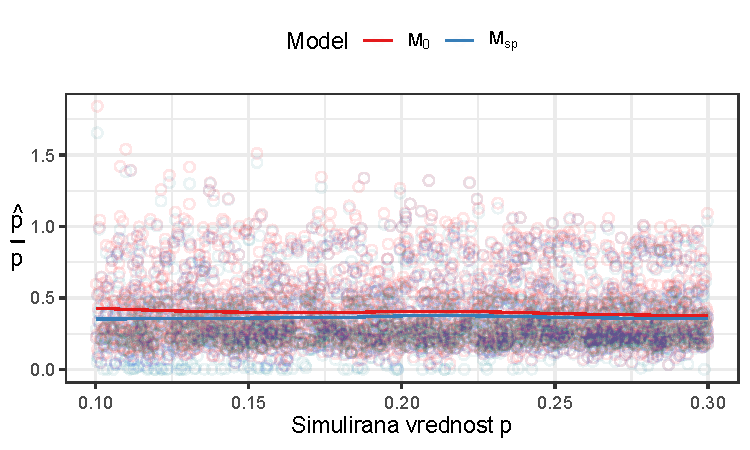
\includegraphics[width=1\linewidth]{C:/Users/romunov/Documents/workspace/doktorat/analiza/figures/E-0a_pristranskost_1_in_sp_ocene_ulovljivosti.pdf}
  \label{sli:sub3.1}
\end{subfigure}

\begin{subfigure}[b]{0.75\textwidth}
  \centering
  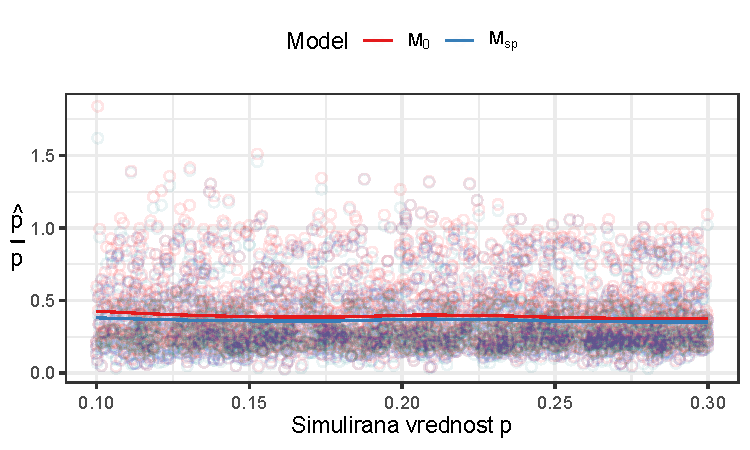
\includegraphics[width=1\linewidth]{C:/Users/romunov/Documents/workspace/doktorat/analiza/figures/N-0a_pristranskost_1_in_sp_ocene_ulovljivosti.pdf}
  \label{sli:sub3.2}
\end{subfigure}

\caption[Primerjava ocenjene ulovljivosti s simulirano]{Povprečna ocena ulovljivosti (parameter $p$) za Hugginsova modela $M_0$ in $M_{sp}$. Na osi $x$ so prikazane simulirane vrednosti $p$, na osi $y$ pa razmerje med ocenjeno in simulirano vrednostjo. V primeru, da ne bi bilo kršenih predpostavk, bi morala biti ocena in simulirana vrednost približno podobni (in njuno razmerje $\sim 1$). Izračun individualne spremenljivke s pomočjo empirične (zgoraj) in normalne funkcije (spodaj). Ne kaže, da izbira funkcije za izračun individualne spremenljivke bistveno vpliva na oceno parametra $p$.}
\label{sli:slika3}
\end{figure}

\subsubsection{Primerjava ulovljivosti glede na število simuliranih osebkov}
Ocena ulovljivosti ($p$) glede na število simuliranih osebkov kaže podobno sliko (slika \ref{sli:slika4}). V povprečju model, kjer smo uporabili za izračun še individualno spremenljivko ($M_{sp}$), bolj podcenjuje ulovljivost kot model brez nje ($M_0$). Ta razlika je relativno majhna.

Opazili smo tudi trend, da je razkorak med modeloma večji za simulacije z manj osebki za manjše simulirane ulovljivosti. Z večanjem simuliranega parametra p se razlika zmanjšuje tudi za primere z najmanjšim številom simuliranih osebkov. Razlike med simulacijami, kjer smo individualno spremenljivko izračunali s pomočjo empirične ali normalne porazdelitve, so relativno majhne.

\begin{figure}[H]
\centering
\begin{subfigure}[b]{1\textwidth}
  \centering
  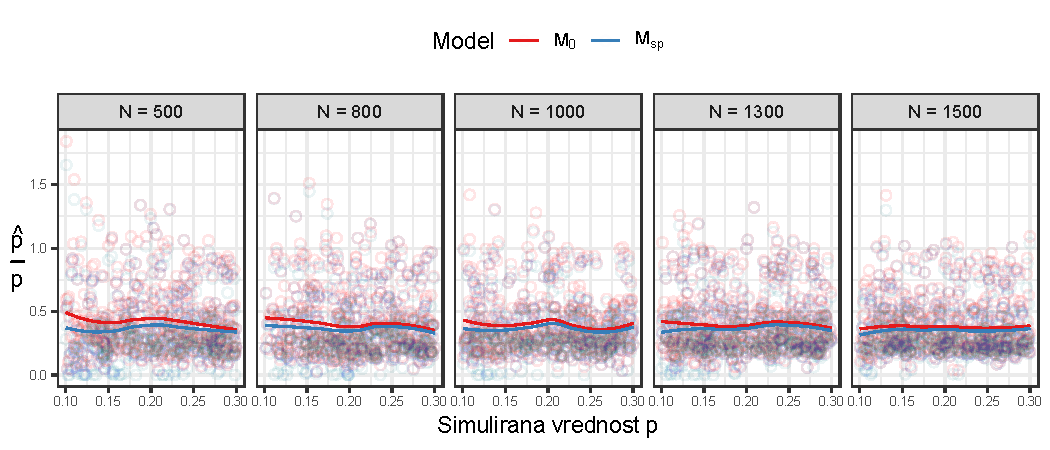
\includegraphics[width=1\linewidth]{C:/Users/romunov/Documents/workspace/doktorat/analiza/figures/E-0b_pristranskost_p1_in_psp_glede_na_st_walkerjev.pdf}

  \label{sli:sub4.1}
\end{subfigure}

\begin{subfigure}[b]{1\textwidth}
  \centering
  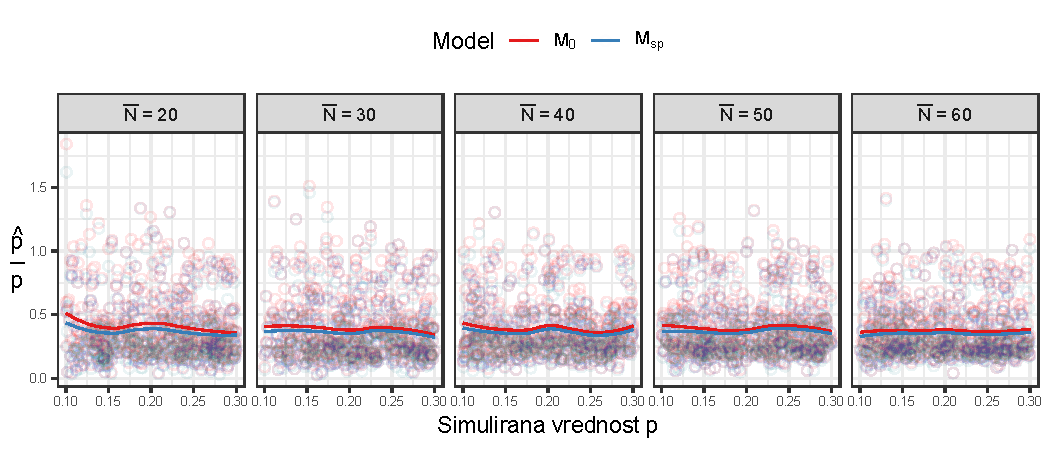
\includegraphics[width=1\linewidth]{C:/Users/romunov/Documents/workspace/doktorat/analiza/figures/N-0b_pristranskost_p1_in_psp_glede_na_st_walkerjev.pdf}
  \label{sli:sub4.2}
\end{subfigure}

\caption[Primerjava ocenjene ulovljivosti s simulirano glede na število simuliranih osebkov]{Zgornja slika prikazuje podatke, kjer smo individualno spremenljivko ocenili s pomočjo empirične spremenljivke, spodnja pa podatke za simulacije, kjer smo individualno spremenljivko izračunali s pomočjo normalne porazdelitve. Točke prikazujejo razmerje med oceno ulovljivosti in pravo, simulirano, vrednostjo glede na število generiranih osebkov. Na x osi so prikazane simulirane vrednosti ulovljivosti, na y osi pa razmerje med ocenjeno in simulirano vrednostjo. Okenca prikazujejo podatke glede na število simuliranih osebkov (od 500 do 1500).}
\label{sli:slika4}
\end{figure}

\subsubsection{Primerjava ulovljivosti glede na razmerje velikosti domačega okoliša in območja vzorčenja}
S slike \ref{sli:slika5} je razvidno, da je vpliv zelo velik. Ko je razmerje velikosti domačega okoliša in velikosti območja vzorčenja majhno (majhen domač okoliš v primerjavi z območjem zvorčenja), je ocena parametra relativno zanesljiva. Z večanjem razmerja med domačim okolišem in območjem vzorčenja pa se zanesljivost ocene poslabšuje in se celo spusti pod globalno povprečje.

Sodeč po naših rezultatih s slike \ref{sli:slika5}, ne moremo sklepati, da ima število generiranih osebkov v povezavi z razmerjem domačega okoliša in vzorčenega območja bistven vpliv na oceno ulovljivosti oz. je vpliv neznaten. Razlike med simulacijami, kjer smo spreminjali funkcijo za izračun individualne spremenljivke, so majhne oz. jih ni.

\begin{figure}[H]
\centering
\begin{subfigure}[b]{1\textwidth}
  \centering
  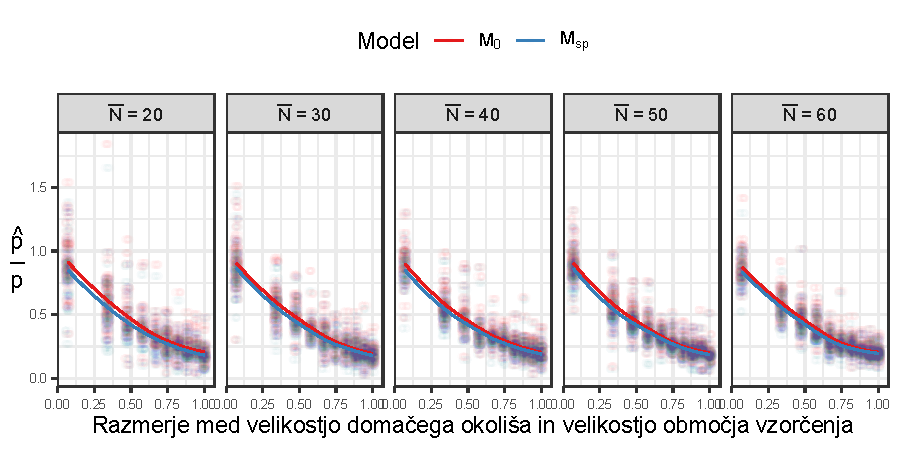
\includegraphics[width=1\linewidth]{C:/Users/romunov/Documents/workspace/doktorat/analiza/figures/E-0f_pristranskost_p_glede_na_sap_hr_ratio_po_st_gen_walkerjev_brez_popravka.pdf}

  \label{sli:sub5.1}
\end{subfigure}

\begin{subfigure}[b]{1\textwidth}
  \centering
  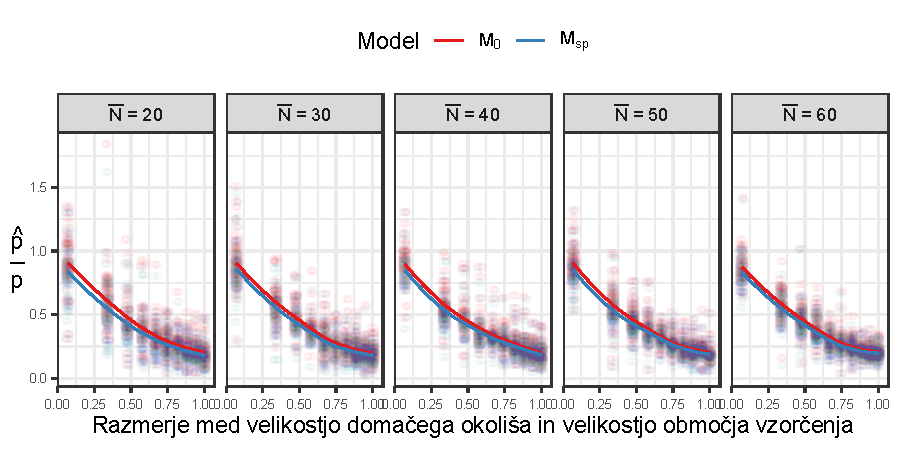
\includegraphics[width=1\linewidth]{C:/Users/romunov/Documents/workspace/doktorat/analiza/figures/N-0f_pristranskost_p_glede_na_sap_hr_ratio_po_st_gen_walkerjev_brez_popravka.pdf}
  \label{sli:sub5.2}
\end{subfigure}

\caption[Vpliv razmerja med ocenjeno in pravo ulovljivostjo v povezavi z razmerjem velikosti domačega okoliša in vzorčenega območja.]{Vpliv razmerja med ocenjeno in pravo ulovljivostjo v povezavi z razmerjem velikosti domačega okoliša in vzorčenega območja. Zgornja slika je za simulacije, kjer smo individualno spremenljivko izračunali s pomočjo empirične porazdelitve, spodnja pa s pomočjo normalne porazdelitve.}
\label{sli:slika5}
\end{figure}

Razmerje med površinama domačega okoliša in območja vzorčenja ima na pristranskost ocene parametra $p$ velik vpliv. Na sliki 6 je prikazano kako se pristranskost ocene parametra $p$ spreminja z razmerjem površin domačega okoliša in vzorčenega območja glede na število generiranih osebkov in odlovnih presledkov. Povprečji ocen obeh Hugginsovih modelov konvergirata z večanjem razmerja, kjer več simuliranih osebkov pomeni bolj podobno (in pristransko) oceno med modeloma. Podoben vpliv ima tudi število odlovnih presledkov, poleg tega pa le-ti vpliva tudi na variabilnost ocen. Več kot je odlovnih presledkov, manjša je variabilnost v oceni. S slike \ref{sli:slika6} ne moremo trditi, da smo zaznali bistvene razlike med simulacijami, kjer smo za izračun individualne spremenljivke uporabili normalno ali empirično funkcijo.

\begin{figure}[H]
\centering
\begin{subfigure}[b]{1\textwidth}
  \centering
  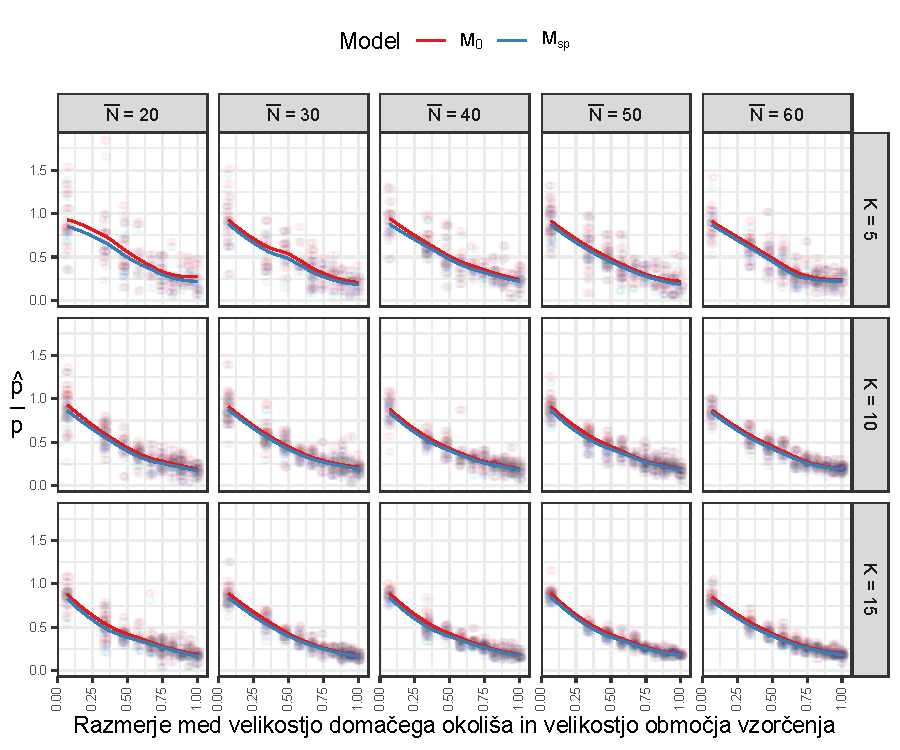
\includegraphics[width=0.8\linewidth]{C:/Users/romunov/Documents/workspace/doktorat/analiza/figures/E-0h_pristranskost_p_glede_sap_hr_razmerje_glede_na_st_walkerjev_in_st_sessionov.pdf}
  \label{sli:sub6.1}
\end{subfigure}

\begin{subfigure}[b]{1\textwidth}
  \centering
  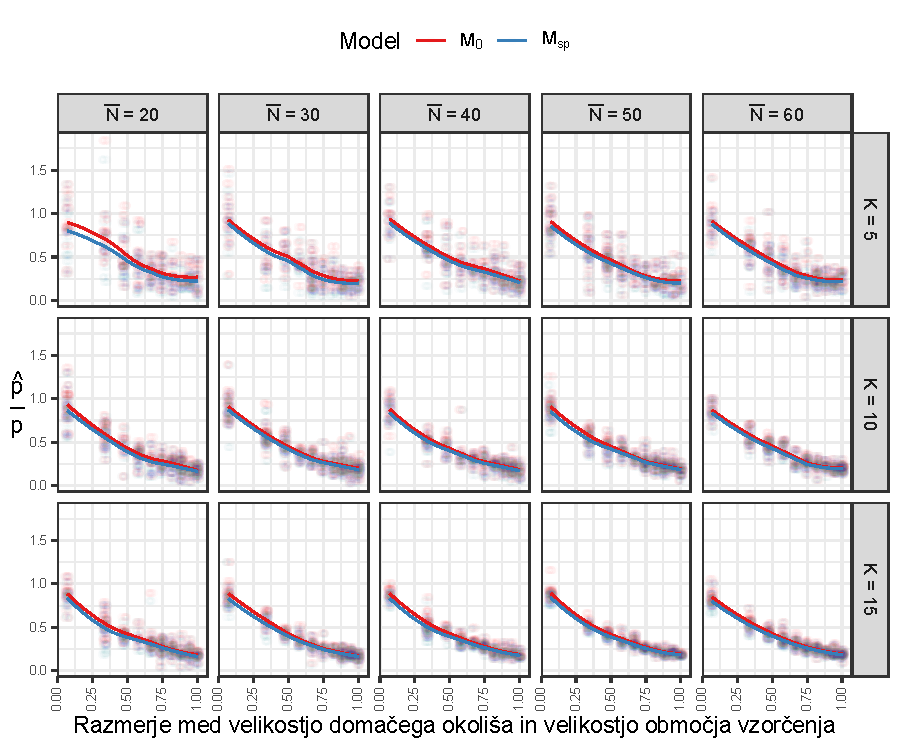
\includegraphics[width=0.8\linewidth]{C:/Users/romunov/Documents/workspace/doktorat/analiza/figures/N-0h_pristranskost_p_glede_sap_hr_razmerje_glede_na_st_walkerjev_in_st_sessionov.pdf}
  \label{sli:sub6.2}
\end{subfigure}
\caption[Prikaz pristranskosti ocene ulovljivosti ($p$) glede na razmerje površin domačega okoliša in območja vzorčenja v povezavi s številom simuliranih osebkov (stolpci) in odlovnih presledkov (vrstice).]{Prikaz pristranskosti ocene ulovljivosti ($p$) glede na razmerje površin domačega okoliša in območja vzorčenja v povezavi s številom simuliranih osebkov (stolpci) in odlovnih presledkov (vrstice). Na prvi sliki so prikazani rezultati simulacij, kjer smo za izračun individualne spremenljivke uporabili empirično, na spodnji pa normalno funkcijo. Na osi $x$ je prikazano razmerje od 0 (površina domačega okoliša zelo majhna v primerjavi s površino vzorčenega območja) do 1 (površina domačega okoliša in vzorčenega območja enako velika). Pristranskost ocene parametra $p$ narašča z večanjem razmerja velikosti domačega okoliša in območja vzorčenja. Povprečja ulovljivosti modelov po Hugginsu konvergirajo. Z večanjem števila simuliranih osebkov se manjša tudi razlika v oceni parametra. Podobno sliko vidimo z večanjem števila odlovnih presledkov (vrstice), kjer poleg konvergence povprečij modelov opazimo tudi manjšanje variance ocene.}
\label{sli:slika6}
\end{figure}

\subsection{Gostota}
Dejansko gostoto smo izračunali kot število centroidov (osebkov) znotraj površine, kjer smo jih simulirali. S pomočjo modelov Huggins in TIRM smo dobili oceno številčnosti znotraj območja vzorčenja. Ker so osebki hodili čez mejo vzorčenega območja, smo tako dejansko ocenili velikost superpopulacije katere prostorska omejenost ni nedvoumno določena. Na podlagi ocenjenega števila osebkov in velikosti vzorčenega območja smo izračunali gostoto te superpopulacije. Za izračun gostote smo uporabili tudi razširjeno območje vzorčenja. Območje smo razširili tako, da smo polmer povečali za določeno razdaljo. Razdaljo smo izbrali kot percentil parne razdalje iz funkcije, ki smo jo ali prilegli podatkom (empirična funkcija) ali pa izračunali na podlagi simuliranih parametrov (dvorazsežna normalna porazdelitev). Gostoto smo izračunali glede na območje povečano za standardni odklon polmera simuliranega območja gibanja osebka (hr), za percentil porazdelitve (50-99) oz. za najdaljšo prehojeno razdaljo (effect) v posamezni simulaciji. Spodnji rezultati so podani kot razmerje med ocenjeno in pravo gostoto. Ker gre za razmerje kjer je prava gostota v imenovalcu, se bodo v primeru nepristransko ocenjene gostote vrednosti nahajale blizu 1.

\subsubsection{Razlike v gostoti glede na število simuliranih osebkov in funkcij za izračun individualne spremenljivke}
Na sliki \ref{sli:slika6} so prikazani podatki izračuni gostot. Na sliki uporabimo kazalnik, ki je z gostoto povezan kot razmerje med gostoto izračunano iz ocenjene velikosti populacije in simulirane velikosti populacije ($\hat{D}/D$).

Opazimo razlike med simulacijami, kjer smo uporabili empirično in normalno porazdelitev za izračun individualne spremenljivke. Razlike so predvsem v primerih, kjer smo območje vzorčenja povečani za razdaljo od 50. do 99. percentila. Pristranskost kazalnika se v odvisnosti od razmerja domačega okoliša in vzorčenega območja povečuje hitreje za primere, ko smo za izračun individualne spremenljivke uporabili empirično porazdelitev.

Pristranskost kazalnika v primeru nepovečanega območje hitro narašča z večanjem razmerja med velikostjo domačega okoliša in velikostjo območja vzorčenja podobno za oba načina izračuna individualne spremenljivke.

Z manjšanjem razmerja med površino domačega okoliša in območja vzorčenja se pristranskost v povprečju zmanjšuje. Za primere, kjer smo za izračun individualne spremenljivke uporabili empirično funkcijo, je gladilka za večja povečanja razmerja bolj konkavne oblike, s povečevanjem površine vzorčenega območja za izračun gostote pa se pristranskost v splošnem zmanjšuje.

Pri simulacijah, kjer smo za izračun individualne spremenljivke uporabili normalno porazdelitev je konkavnosti  možno opaziti le za primere, kjer smo območje vzorčenja povečali za najdaljšo prehojeno razdaljo (zadnji stolpec).
Za oba načina izračuna individualnih spremenljivk pa velja, da se povečanje površine vzorčenega območja pozna najmanj za tiste simulacije, kjer je bilo razmerje med velikostjo domačega okoliša in velikostjo vzorčenega območja najmanjše.

Povečevanje števila simuliranih osebkov prispeva predvsem k zmanjšanju variabilnosti ocen velikosti populacij in posledično k manjši variabilnosti gostot. Variabilnost je za veliko večino primerov najmanjša za simulacije, kjer je razmerje med velikostjo domačega okoliša in velikostjo vzorčenega območja najmanjša.

Razlike med modeli so med scenariji primerljivi. Najbolj precenjene rezultate da model TIRM, manj $M_{sp}$ in najmanj $M_0$. Razlike med modeli izginejo predvsem na račun povečanja razmerja med površinama domačega okoliša in območja vzorčenja.

\begin{figure}[H]
  \centering
  \begin{subfigure}[b]{1\textwidth}
    \centering
    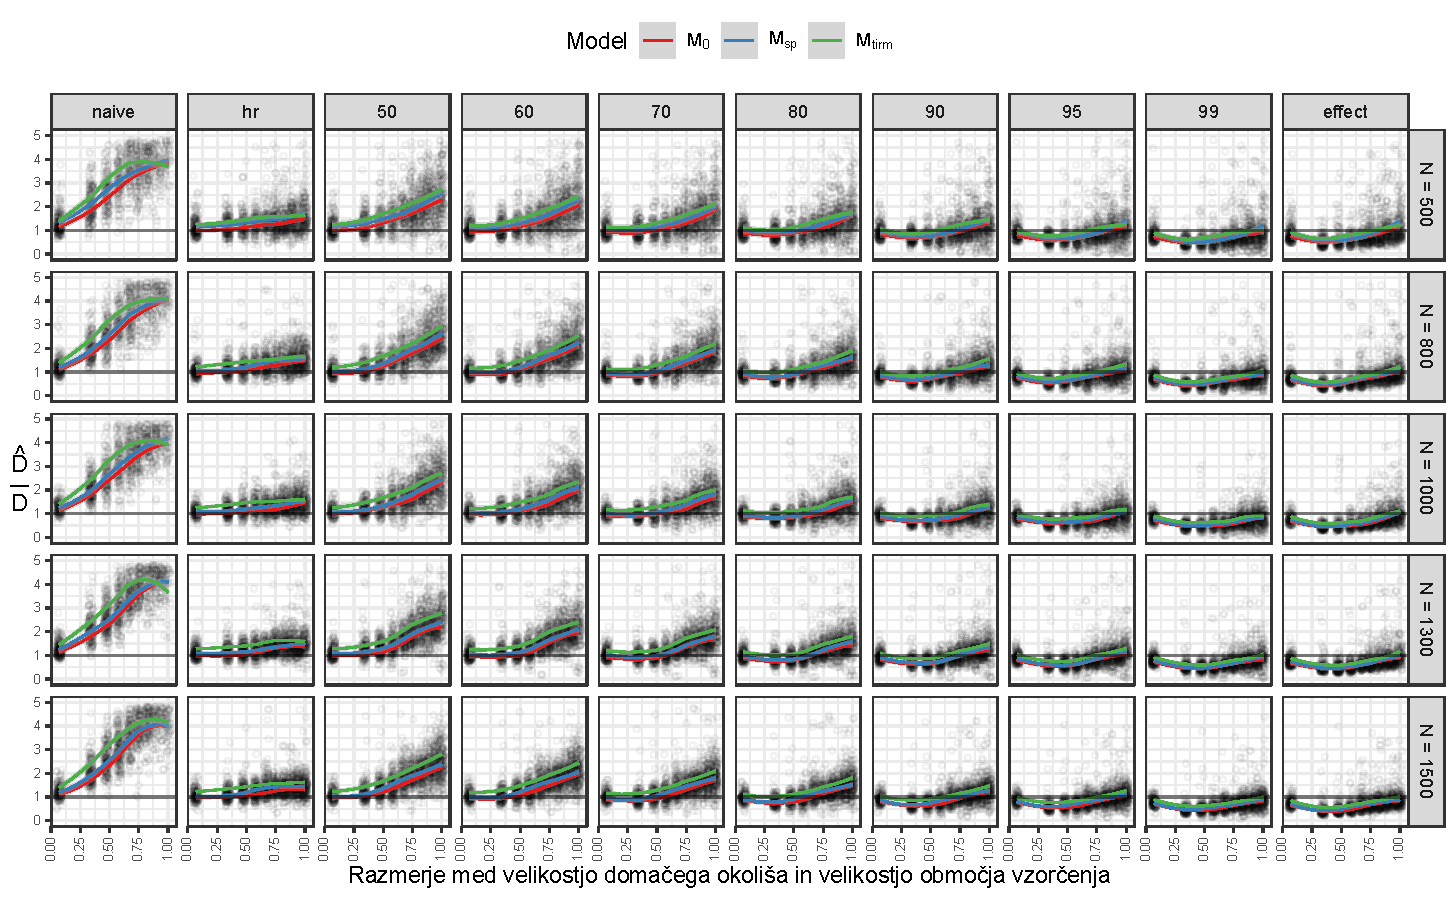
\includegraphics[width=1\linewidth]{C:/Users/romunov/Documents/workspace/doktorat/analiza/figures/E-1a_gostota_gled_na_razmerje_hr_sap_po_correction_type_in_st_gen_walk.pdf}
    \label{sli:sub7.1}
  \end{subfigure}

  \begin{subfigure}[b]{1\textwidth}
    \centering
    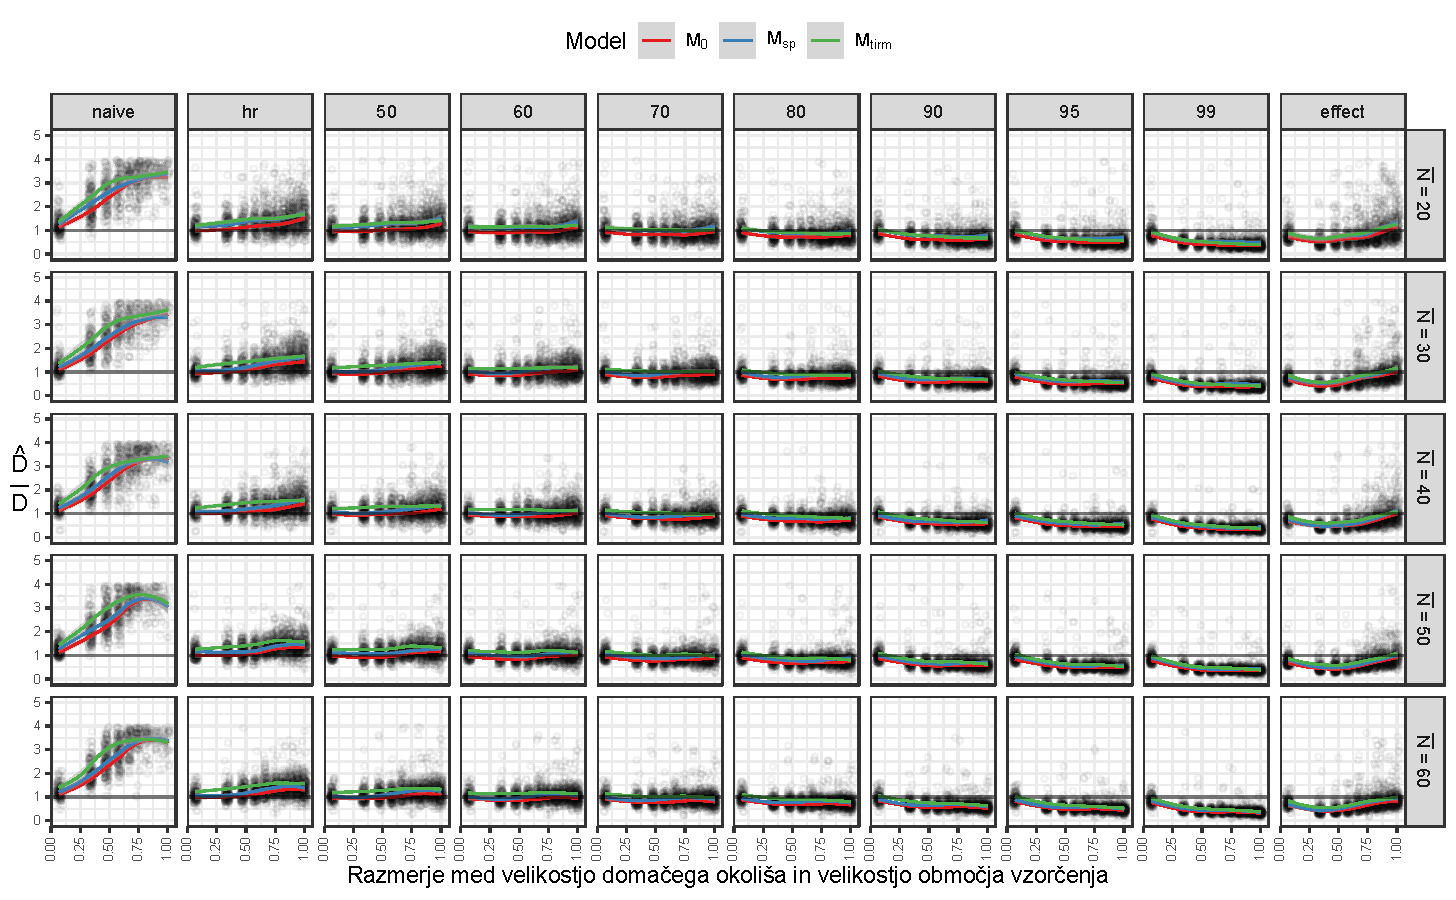
\includegraphics[width=1\linewidth]{C:/Users/romunov/Documents/workspace/doktorat/analiza/figures/N-1a_gostota_gled_na_razmerje_hr_sap_po_correction_type_in_st_gen_walk.pdf}
    \label{sli:sub7.2}
  \end{subfigure}
  \caption[Prikaz kazalnika gostot ($\hat{D}/D$)]{Prikaz kazalnika gostot ($\hat{D}/D$). Na zgornji sliki so prikazani rezultati za simulacije, kjer smo za izračun individualne spremenljivke uporabili empirično porazdelitev, na spodnji pa dvorazsežno normalno porazdelitev. Stolpci oken ponazarjajo razširitev vzorčenega območja za percentil dane porazdelitve, vrstice pa število simuliranih osebkov, na podlagi katerih smo izvedli vzorčenje in posledično izračun velikosti populacije in gostote. Pri izračunu smo uporabili tri modele, Hugginsov model $H_0$, $H_{sp}$, kjer smo ulovljivost modelirali glede na individualno spremenljivko in TIRM, ki predpostavlja dve skupini z različno ulovljivostjo.}
  \label{sli:slika7}
\end{figure}

\subsubsection{Razlike v gostoti glede na funkcijo za izračun individualne spremenljivke, števila odlovnih intervalov ter število simuliranih osebkov}
Na slikah \ref{sli:slika7} in \ref{sli:slika8} smo podatke s slike \ref{sli:slika6} prikazali tako, da so podatki razdeljeni na odlovne presledke ($K = [5, 10, 15]$). Pogled glede na število odlovnih presledkov nam je dal predvsem vpogled v spremembo variabilnosti. Pri simulacijah z najnižjim $K$ ($K = 5$) je varianca večja kot pri tistih s $K = [10, 15]$. Pri slednjih že opazimo prevladujoč vzorec v povprečju kazalnika za vse modele glede na popravke velikosti območja vzorčenja (stolpci) in število simuliranih osebkov (vrstice). Vpliv povečanja površine vzorčenega območja se opazi predvsem za simulacije, kjer je razmerje med velikostjo domačega okoliša in velikostjo vzorčenega območja relativno velika. Na simulacije, kjer je to razmerje relativno majhno, povečanje območja vzorčenja pri pristranskosti ne kaže očitnega učinka.

\begin{figure}[H]
  \centering
  \begin{subfigure}[b]{1\textwidth}
    \centering
    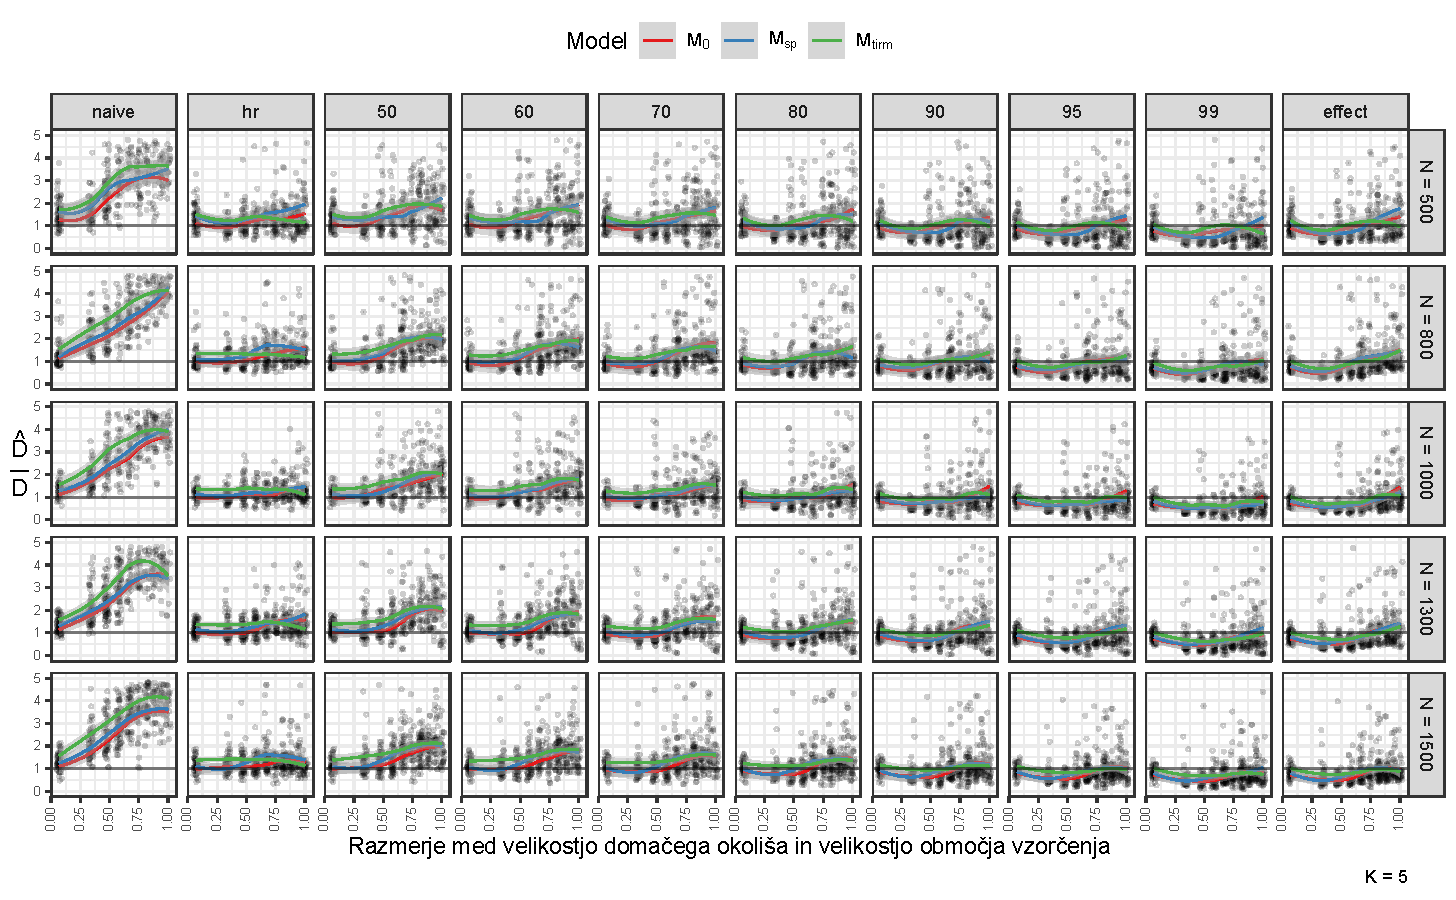
\includegraphics[width=1\linewidth]{C:/Users/romunov/Documents/workspace/doktorat/analiza/figures/E-1c_gostota_gled_na_razmerje_hr_sap_po_correction_type_in_st_gen_walk_za_k5.pdf}
    \label{sli:sub8.1}
  \end{subfigure}

  \begin{subfigure}[b]{1\textwidth}
    \centering
    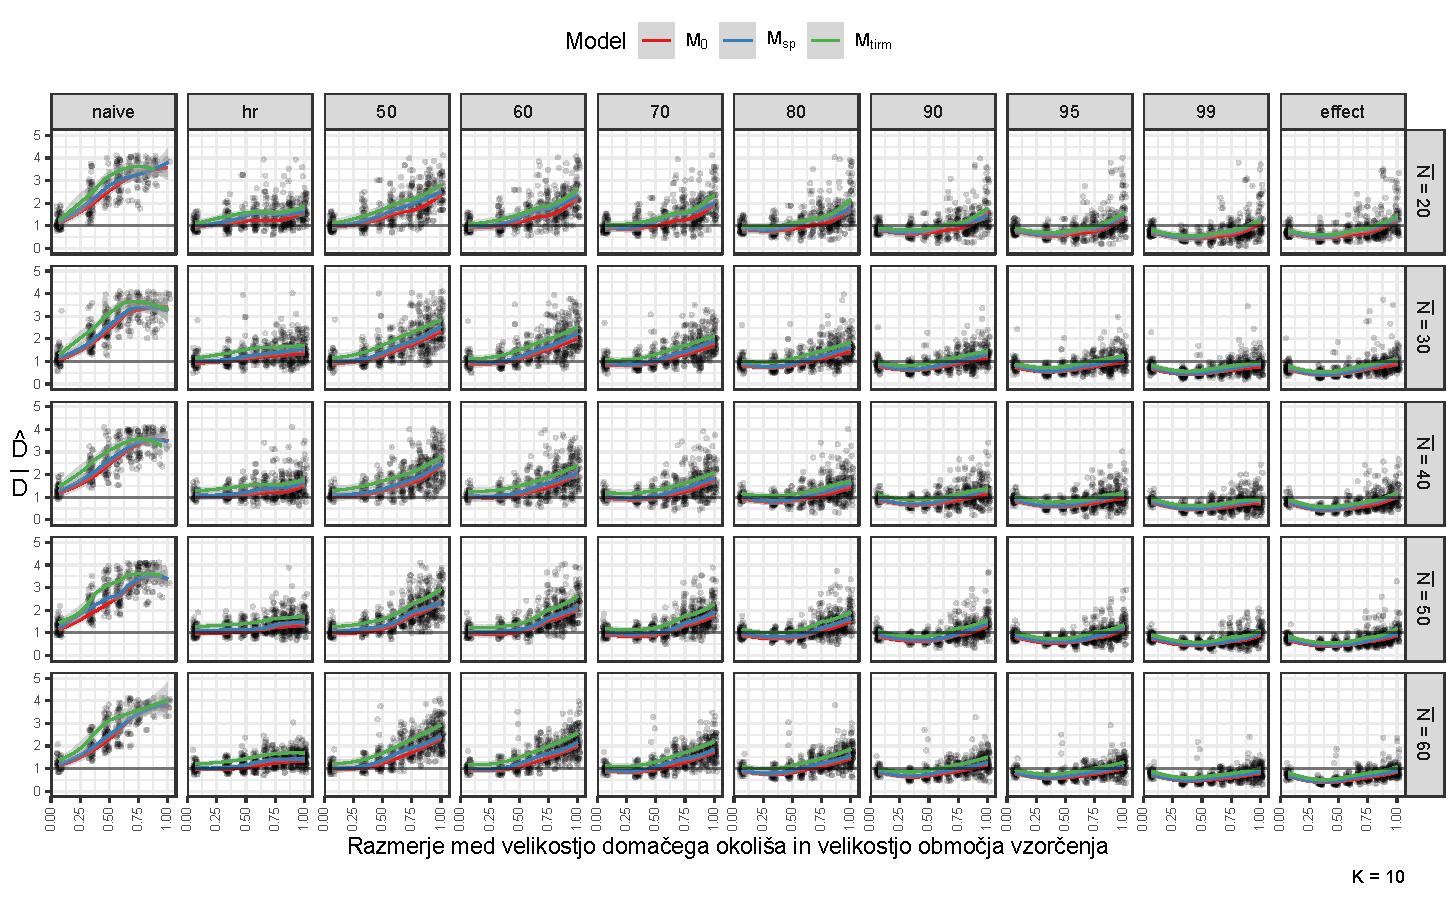
\includegraphics[width=1\linewidth]{C:/Users/romunov/Documents/workspace/doktorat/analiza/figures/E-1d_gostota_glede_na_razmerje_hr_sap_po_correction_type_in_st_gen_walk_za_k10.pdf}
    \label{sli:sub8.2}
  \end{subfigure}
\end{figure}

\begin{figure}[H]
  \ContinuedFloat
  \begin{subfigure}[b]{1\textwidth}
    \centering
    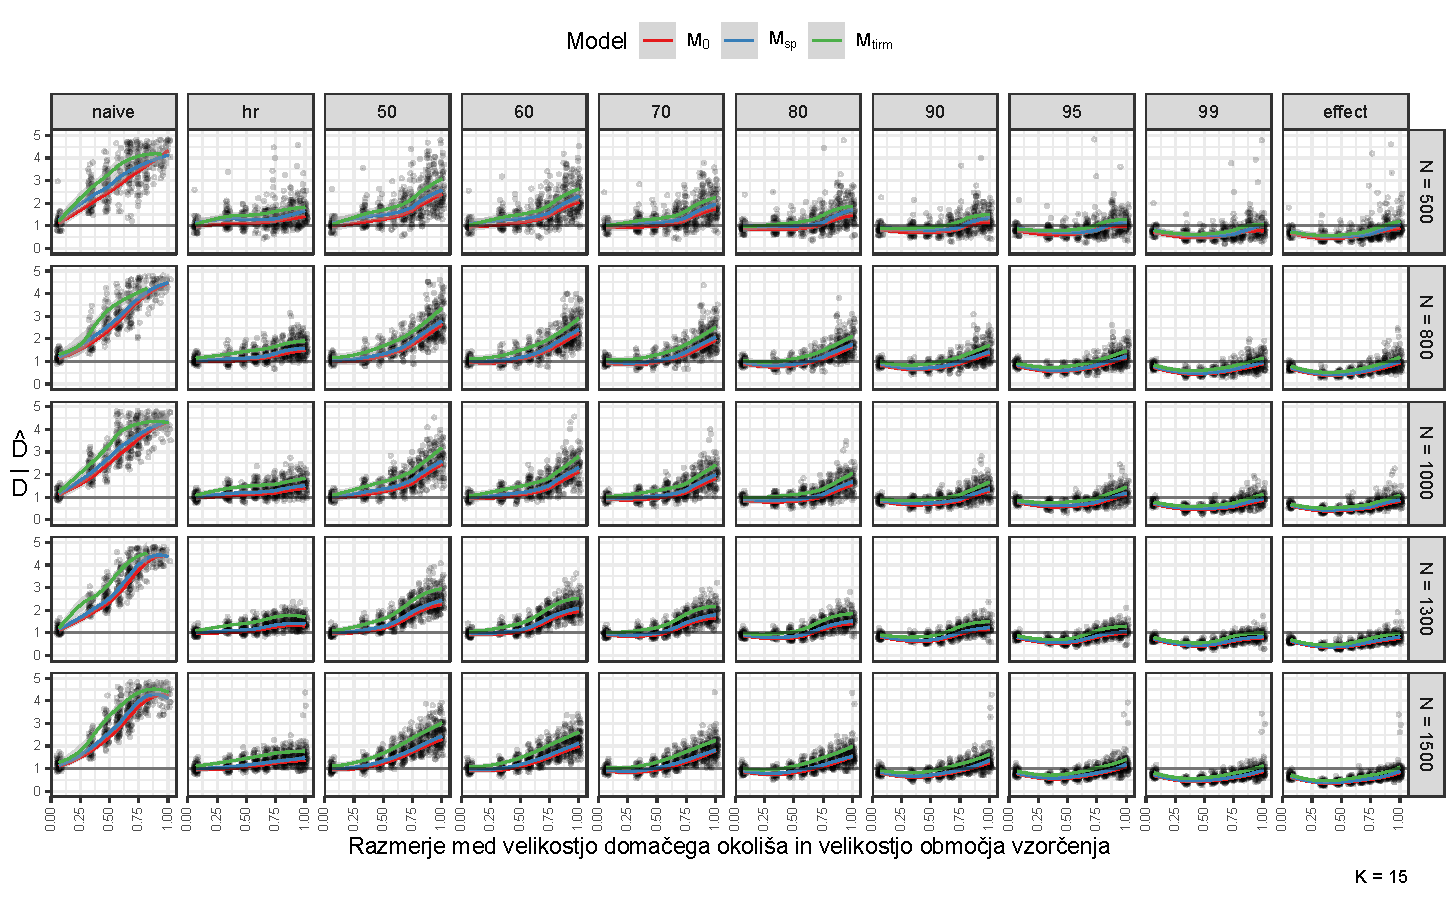
\includegraphics[width=1\linewidth]{C:/Users/romunov/Documents/workspace/doktorat/analiza/figures/E-1e_gostota_glede_na_razmerje_hr_sap_po_correction_type_in_st_gen_walk_za_k15.pdf}
    \label{sli:sub8.3}
  \end{subfigure}
  \caption[Prikaz vrednosti simulacij, kjer smo za izračun individualne spremenljivke uporabili empirično porazdelitev]{Prikaz vrednosti simulacij, kjer smo za izračun individualne spremenljivke uporabili empirično porazdelitev. Ta slika prikazuje iste podatke, kot so na sliki 7 (zgoraj), dodatno pa smo jih razrezali glede na število odlovnih intervalov ($K$). Zgoraj $K=5$, v sredini $K=10$, spodaj $K=15$.}
  \label{sli:slika8}
\end{figure}

\begin{figure}[H]
  \ContinuedFloat
  \centering
  \begin{subfigure}[b]{1\textwidth}
    \centering
    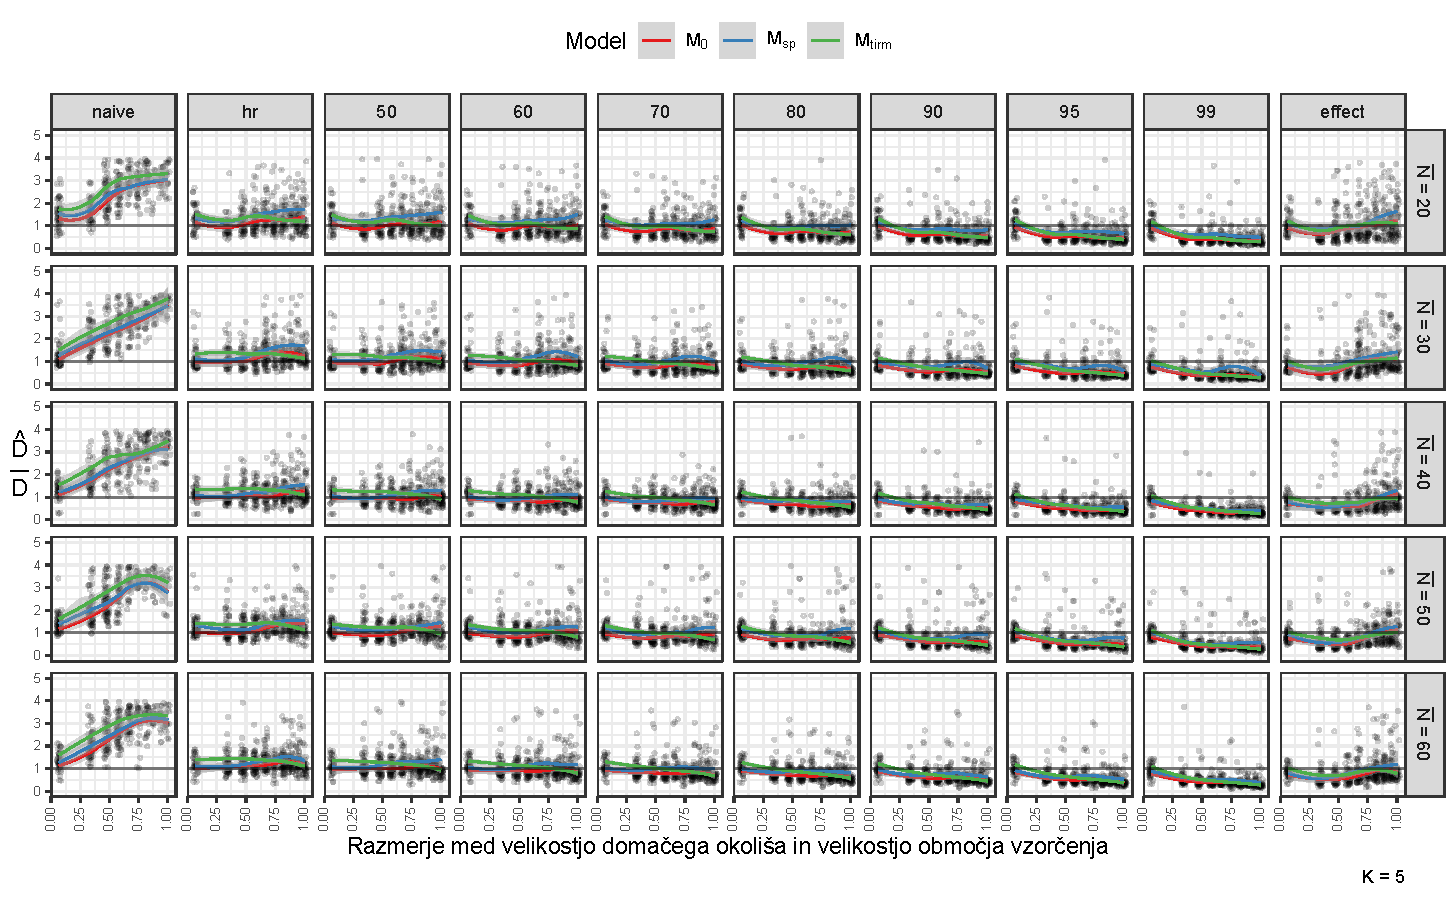
\includegraphics[width=1\linewidth]{C:/Users/romunov/Documents/workspace/doktorat/analiza/figures/N-1c_gostota_gled_na_razmerje_hr_sap_po_correction_type_in_st_gen_walk_za_k5.pdf}
    \label{sli:sub9.1}
  \end{subfigure}

  \begin{subfigure}[b]{1\textwidth}
    \centering
    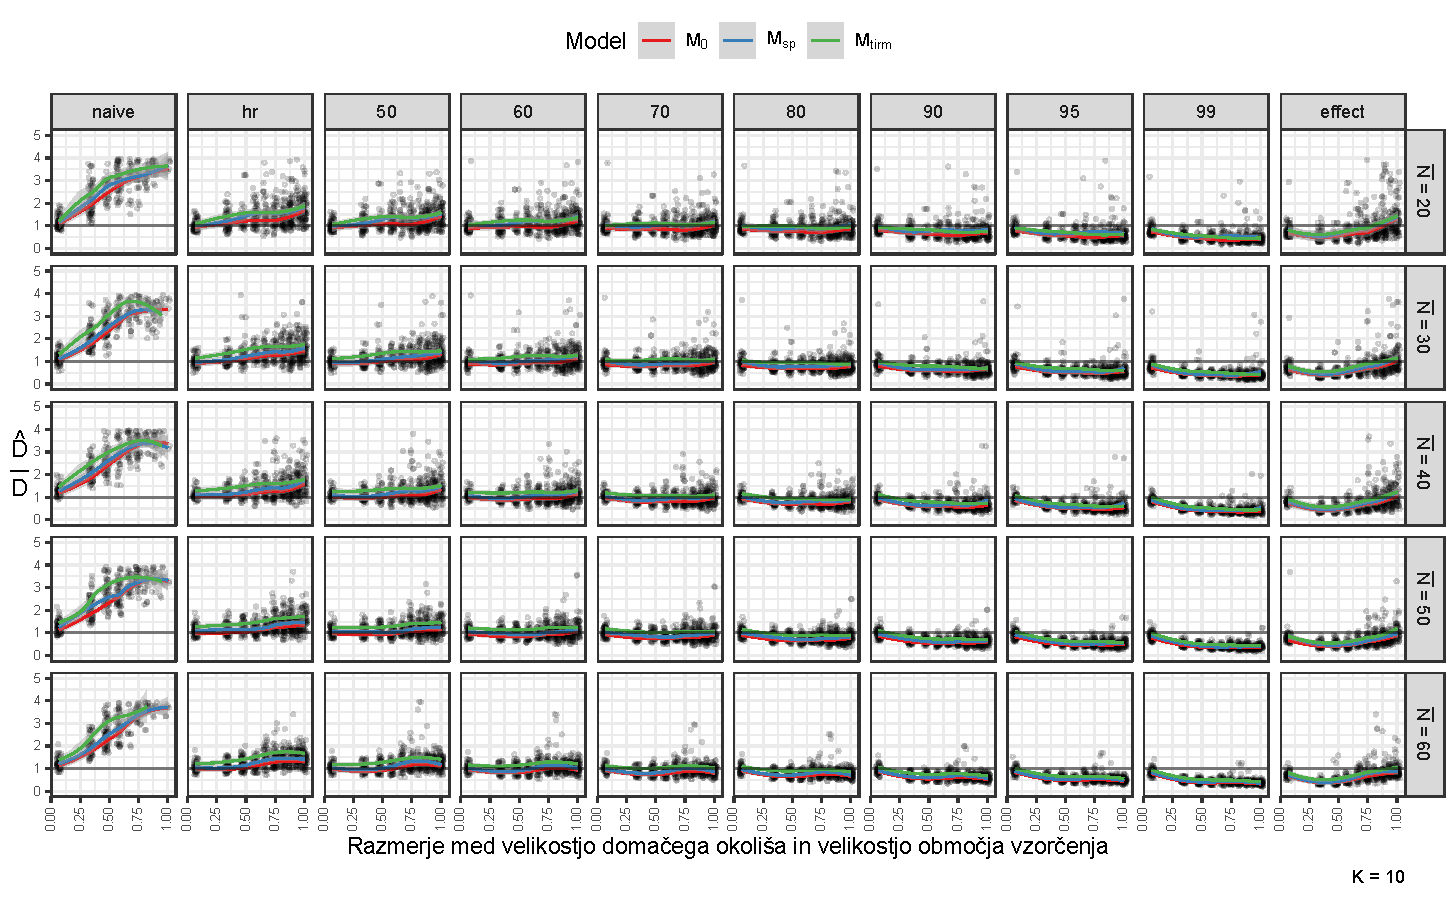
\includegraphics[width=1\linewidth]{C:/Users/romunov/Documents/workspace/doktorat/analiza/figures/N-1d_gostota_glede_na_razmerje_hr_sap_po_correction_type_in_st_gen_walk_za_k10.pdf}
    \label{sli:sub9.2}
  \end{subfigure}
\end{figure}

\begin{figure}[H]
  \ContinuedFloat
  \begin{subfigure}[b]{1\textwidth}
    \centering
    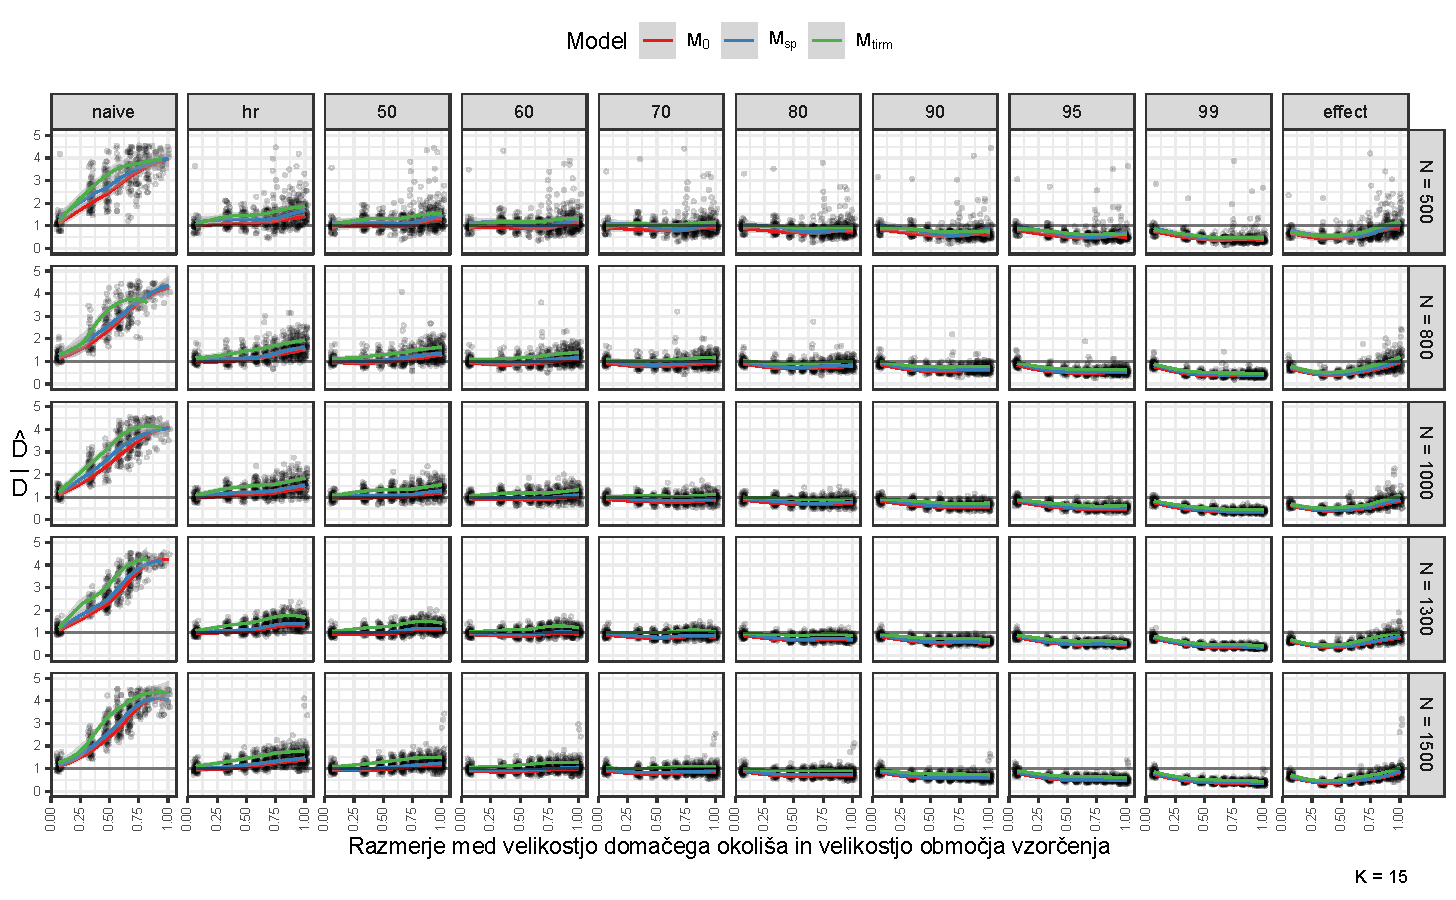
\includegraphics[width=1\linewidth]{C:/Users/romunov/Documents/workspace/doktorat/analiza/figures/N-1e_gostota_glede_na_razmerje_hr_sap_po_correction_type_in_st_gen_walk_za_k15.pdf}
    \label{sli:sub9.3}
  \end{subfigure}
  \caption[Prikaz vrednosti simulacij, kjer smo za izračun individualne spremenljivke uporabili normalno porazdelitev]{Prikaz vrednosti simulacij, kjer smo za izračun individualne spremenljivke uporabili normalno porazdelitev. Ta slika prikazuje iste podatke, kot so na sliki 8 (spodaj), dodatno pa smo jih razrezali glede na število odlovnih intervalov ($K$). Zgoraj $K=5$, v sredini $K=10$, spodaj $K=15$.}
  \label{sli:slika9}
\end{figure}

\subsection{AICc}
Metriko AICc smo primerjali samo za Hugginsova modela M0 in Msp. Verjetje modela TIRM ni primerljiv s Hugginsovim modelom. Poleg tega uporabi za izračun velikosti populacije drugačen set podatkov. Primerjava vrednosti AICc z ostalima dvema modeloma zato ne bi bila pravilna.

Za vsako simulacijo smo določili kateri model ima manjši AICc, nato pa razliko med modeloma prikazali na osi y. Vedno smo odšteli AICc modela M0 od AICc modela Msp. Negativne vrednosti so povezane s tistimi simulacijami, kjer je bil boljši model M0, pozitivne pa kjer je bil boljši model Msp. Če je bil boljši model Msp, je bila razlika pogosto mnogo večja (modra barva) kot v primerih, ko je bil boljši model M0 (rdeča barva). Število simuliranih osebkov ne vplivajo na razliko v AICc (ni prikazano), zato smo podatke prikazali brez te spremenljivke na sliki 10.

\begin{figure}[H]
  \centering
  \begin{subfigure}[b]{1\textwidth}
    \centering
    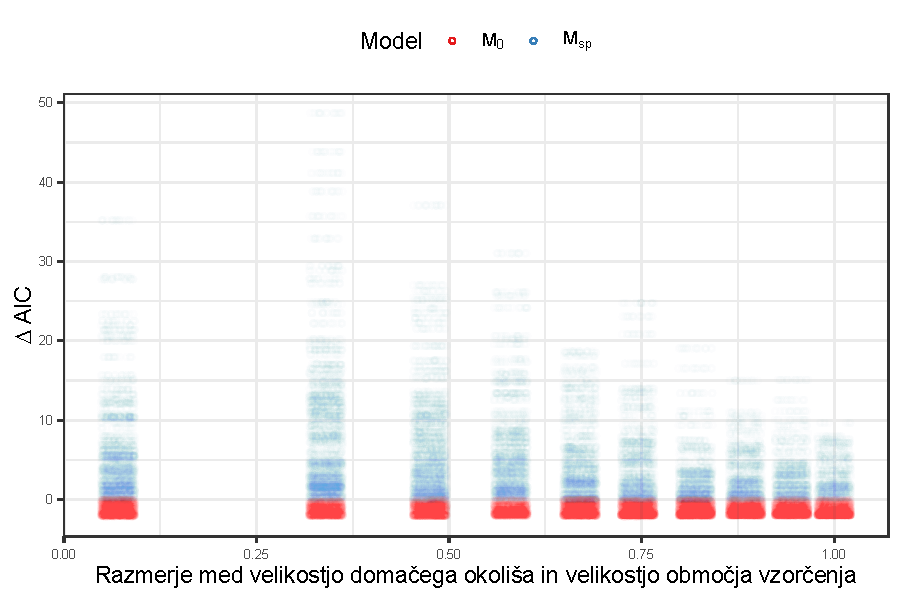
\includegraphics[width=1\linewidth]{C:/Users/romunov/Documents/workspace/doktorat/analiza/figures/E-6b_dAIC_glede_na_razmerje_hr_sap_po_correction_type_in_st_gen_walk_in_boljsi_model.pdf}
    \label{sli:sub10.1}
  \end{subfigure}

  \begin{subfigure}[b]{1\textwidth}
    \centering
    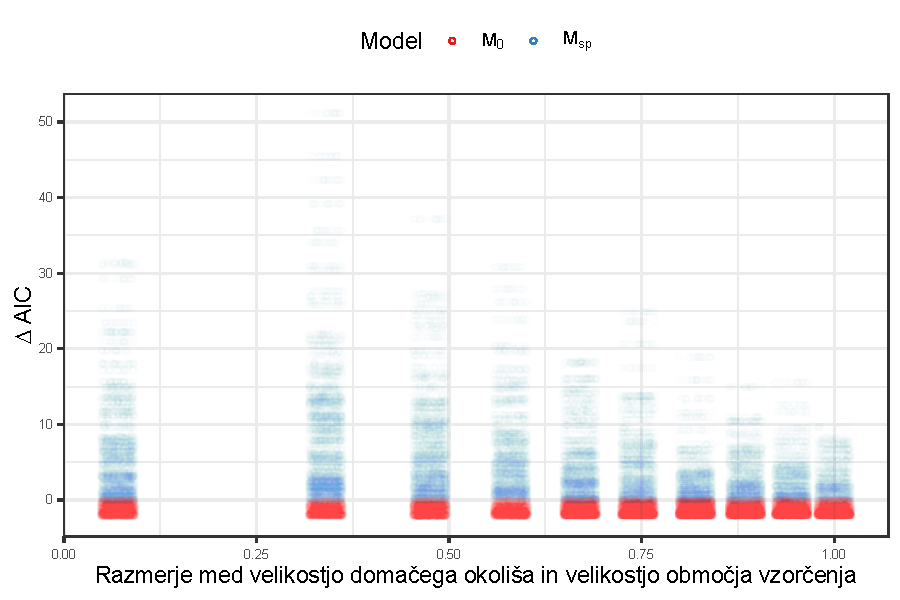
\includegraphics[width=1\linewidth]{C:/Users/romunov/Documents/workspace/doktorat/analiza/figures/N-6b_dAIC_glede_na_razmerje_hr_sap_po_correction_type_in_st_gen_walk_in_boljsi_model.pdf}
    \label{sli:sub10.2}
  \end{subfigure}
  \caption[Prikaz razlike v AICc za modela $M_0$ in $M_{sp}$]{Prikaz razlike v AICc za modela $M_0$ in $M_{sp}$. Na zgornji sliki so prikazani podatki, ker smo za izračun individualne spremenljivke uporabili empirično porazdelitev, na spodnji pa normalno porazdelitev. Rdeče obarvane točke predstavljajo simulacije, kjer je bil boljši model $M_0$, modre pa $M_{sp}$.}
  \label{sli:slika10}
\end{figure}

Porazdelitev vrednosti so nekoliko bolj razvidne s slike 11. Opazimo, da glede na to katero porazdelitev uporabimo za izračun individualne spremenljivke, v rezultatih ni razlik.

\begin{figure}[H]
  \centering
  \begin{subfigure}[b]{1\textwidth}
    \centering
    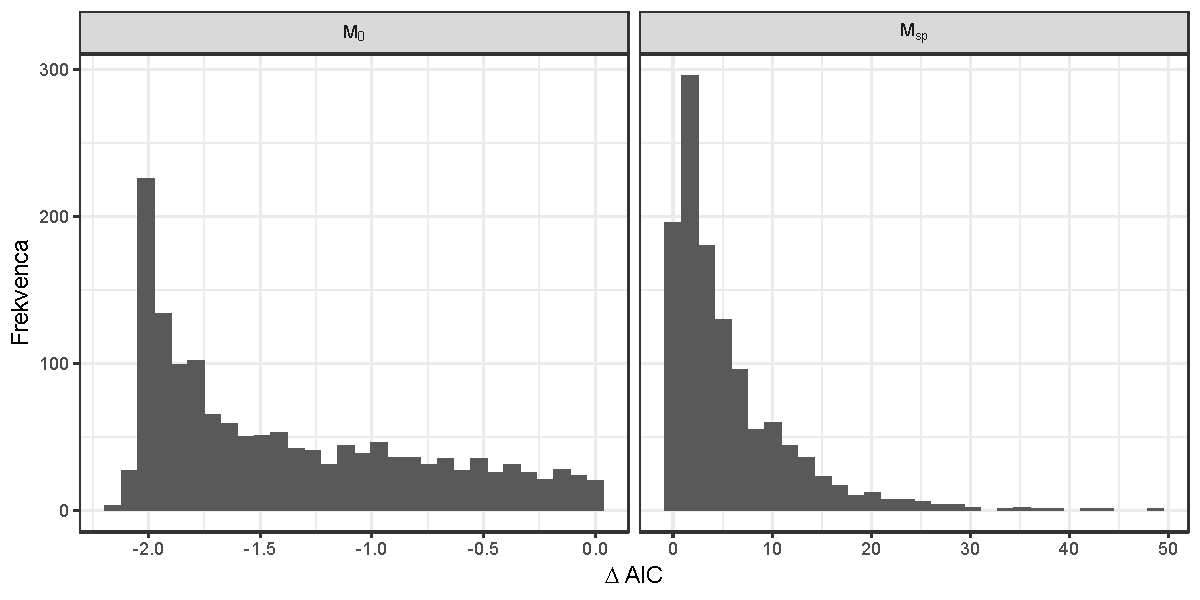
\includegraphics[width=1\linewidth]{C:/Users/romunov/Documents/workspace/doktorat/analiza/figures/E-8a_dAIC_glede_na_najboljsi_model.pdf}
    \label{sli:sub11.1}
  \end{subfigure}

  \begin{subfigure}[b]{1\textwidth}
    \centering
    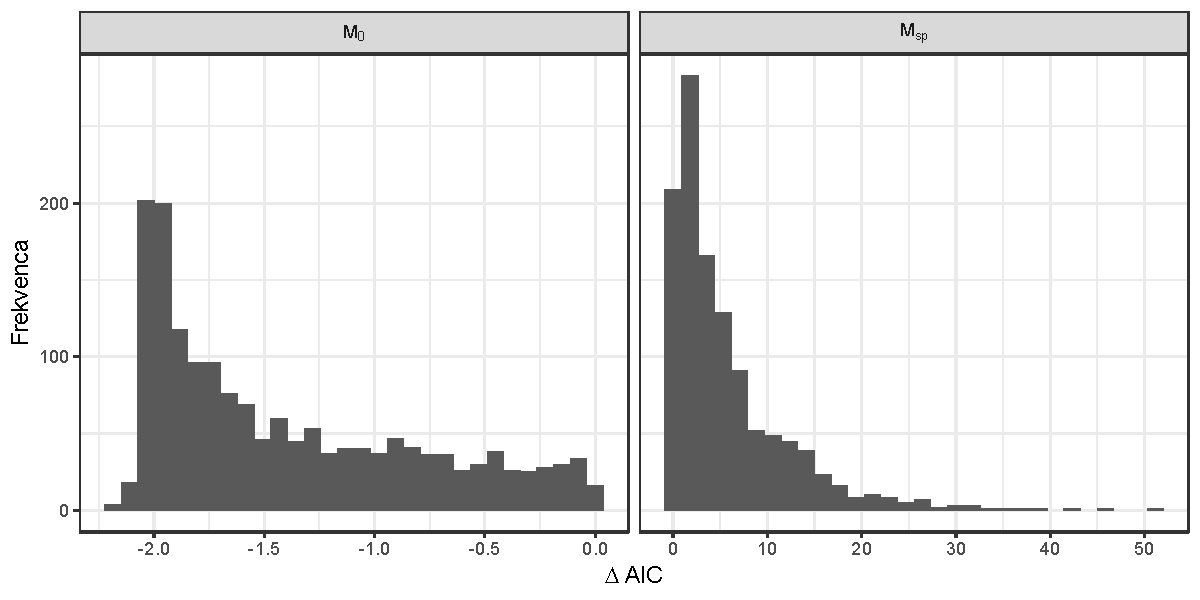
\includegraphics[width=1\linewidth]{C:/Users/romunov/Documents/workspace/doktorat/analiza/figures/N-8a_dAIC_glede_na_najboljsi_model.pdf}
    \label{sli:sub11.2}
  \end{subfigure}
  \caption[Prikaz razlike v AICc za modela $M_0$ in $M_{sp}$]{Porazdelitev razlik v AICc za modela $M_0$ in $M_{sp}$ s slike 10. Zgornja dva histograma predstavljata vrednosti, kjer smo za izračun individualnih spremenljivk uporabili empirično porazdelitev, spodnja dva pa normalno porazdelitev. Previdni morami biti  pri razlaganju osi x, saj le-ti med modeloma nista primerljivi.}
  \label{sli:slika11}
\end{figure}
